\documentclass[14pt]{extbook}
\usepackage{multicol, enumerate, enumitem, hyperref, color, soul, setspace, parskip, fancyhdr} %General Packages
\usepackage{amssymb, amsthm, amsmath, bbm, latexsym, units, mathtools} %Math Packages
\everymath{\displaystyle} %All math in Display Style
% Packages with additional options
\usepackage[headsep=0.5cm,headheight=12pt, left=1 in,right= 1 in,top= 1 in,bottom= 1 in]{geometry}
\usepackage[usenames,dvipsnames]{xcolor}
\usepackage{dashrule}  % Package to use the command below to create lines between items
\newcommand{\litem}[1]{\item#1\hspace*{-1cm}\rule{\textwidth}{0.4pt}}
\pagestyle{fancy}
\lhead{Progress Quiz 3}
\chead{}
\rhead{Version B}
\lfoot{}
\cfoot{}
\rfoot{Fall 2020}
\begin{document}

\begin{enumerate}
\litem{
Choose the equation of the function graphed below.
\begin{center}
    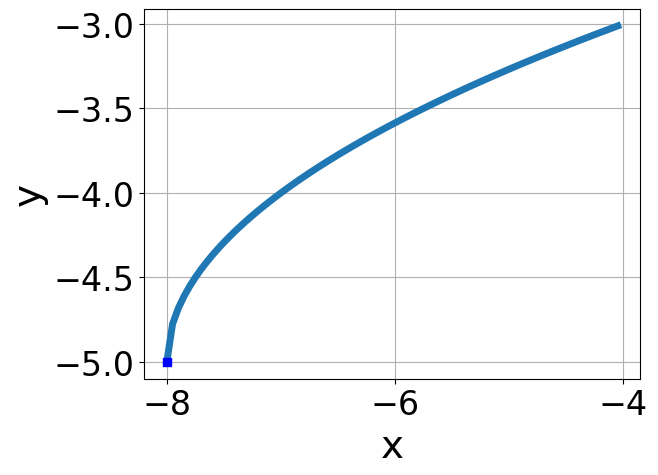
\includegraphics[width=0.5\textwidth]{../Figures/radicalGraphToEquationCopyB.png}
\end{center}
\begin{enumerate}[label=\Alph*.]
\item \( f(x) = - \sqrt[3]{x + 8} - 5 \)
\item \( f(x) = \sqrt[3]{x + 8} - 5 \)
\item \( f(x) = \sqrt[3]{x - 8} - 5 \)
\item \( f(x) = - \sqrt[3]{x - 8} - 5 \)
\item \( \text{None of the above} \)

\end{enumerate} }
\litem{
Choose the equation of the function graphed below.
\begin{center}
    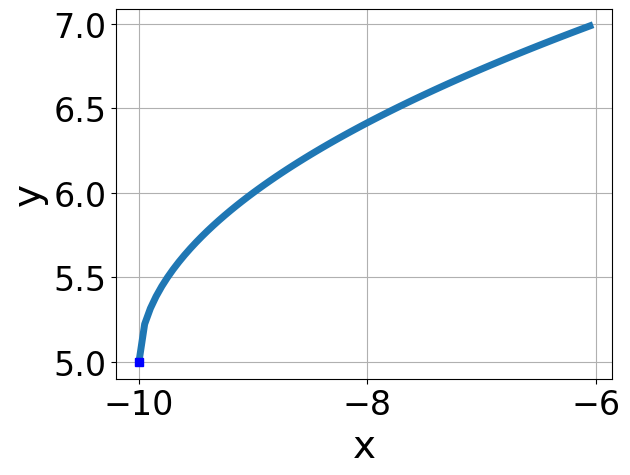
\includegraphics[width=0.5\textwidth]{../Figures/radicalGraphToEquationB.png}
\end{center}
\begin{enumerate}[label=\Alph*.]
\item \( f(x) = - \sqrt{x + 14} + 3 \)
\item \( f(x) = \sqrt{x - 14} + 3 \)
\item \( f(x) = \sqrt{x + 14} + 3 \)
\item \( f(x) = - \sqrt{x - 14} + 3 \)
\item \( \text{None of the above} \)

\end{enumerate} }
\litem{
What is the domain of the function below?\[ f(x) = \sqrt[5]{9 x - 7} \]\begin{enumerate}[label=\Alph*.]
\item \( (-\infty, \infty) \)
\item \( \text{The domain is } [a, \infty), \text{   where } a \in [0.54, 1.21] \)
\item \( \text{The domain is } (-\infty, a], \text{   where } a \in [0.99, 1.68] \)
\item \( \text{The domain is } [a, \infty), \text{   where } a \in [0.92, 1.89] \)
\item \( \text{The domain is } (-\infty, a], \text{   where } a \in [0.38, 0.83] \)

\end{enumerate} }
\litem{
What is the domain of the function below?\[ f(x) = \sqrt[3]{-5 x + 7} \]\begin{enumerate}[label=\Alph*.]
\item \( \text{The domain is } [a, \infty), \text{   where } a \in [-0.29, 0.86] \)
\item \( \text{The domain is } (-\infty, a], \text{   where } a \in [0.45, 0.94] \)
\item \( (-\infty, \infty) \)
\item \( \text{The domain is } [a, \infty), \text{   where } a \in [1.24, 1.63] \)
\item \( \text{The domain is } (-\infty, a], \text{   where } a \in [0.79, 1.94] \)

\end{enumerate} }
\litem{
Solve the radical equation below. Then, choose the interval(s) that the solution(s) belongs to.\[ \sqrt{-7 x + 5} - \sqrt{7 x + 6} = 0 \]\begin{enumerate}[label=\Alph*.]
\item \( x \in [-0.41,0.08] \)
\item \( x_1 \in [-0.41, 0.08] \text{ and } x_2 \in [-2.29,2.71] \)
\item \( x \in [0.33,1.32] \)
\item \( x_1 \in [-0.88, -0.71] \text{ and } x_2 \in [-2.29,2.71] \)
\item \( \text{All solutions lead to invalid or complex values in the equation.} \)

\end{enumerate} }
\litem{
Choose the graph of the equation below.\[ f(x) = - \sqrt[3]{x + 14} + 4 \]\begin{enumerate}[label=\Alph*.]
\begin{multicols}{2}\item 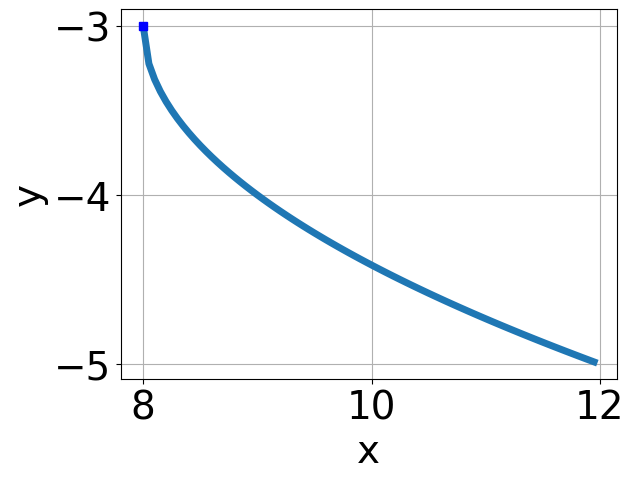
\includegraphics[width = 0.3\textwidth]{../Figures/radicalEquationToGraphCopyAB.png}\item 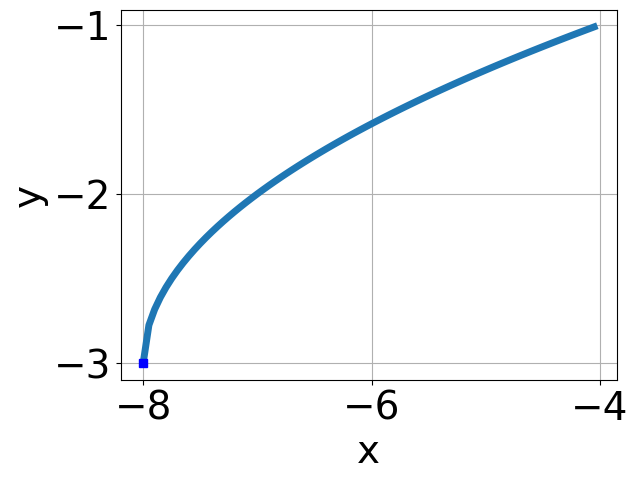
\includegraphics[width = 0.3\textwidth]{../Figures/radicalEquationToGraphCopyBB.png}\item 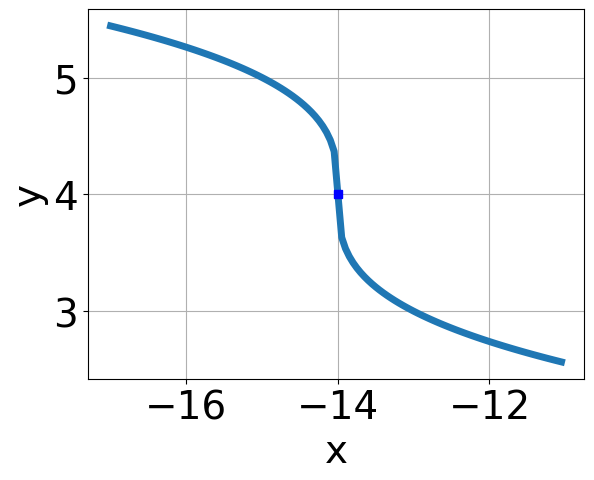
\includegraphics[width = 0.3\textwidth]{../Figures/radicalEquationToGraphCopyCB.png}\item 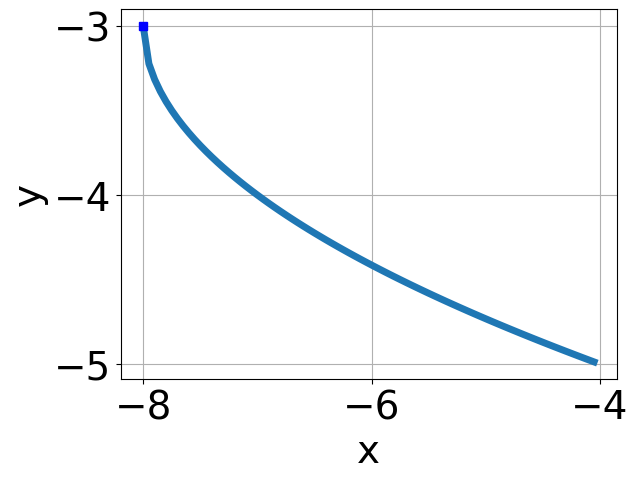
\includegraphics[width = 0.3\textwidth]{../Figures/radicalEquationToGraphCopyDB.png}\end{multicols}\item None of the above.
\end{enumerate} }
\litem{
Choose the graph of the equation below.\[ f(x) = - \sqrt[3]{x + 12} - 7 \]\begin{enumerate}[label=\Alph*.]
\begin{multicols}{2}\item 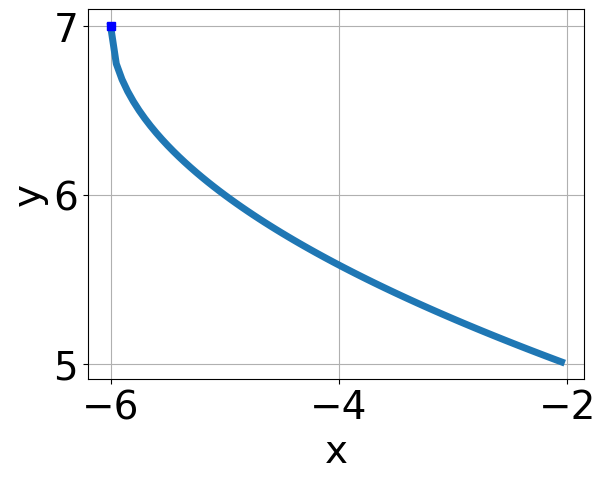
\includegraphics[width = 0.3\textwidth]{../Figures/radicalEquationToGraphAB.png}\item 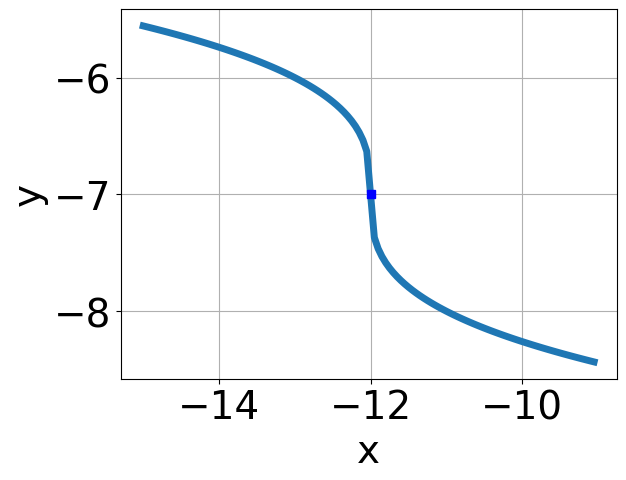
\includegraphics[width = 0.3\textwidth]{../Figures/radicalEquationToGraphBB.png}\item 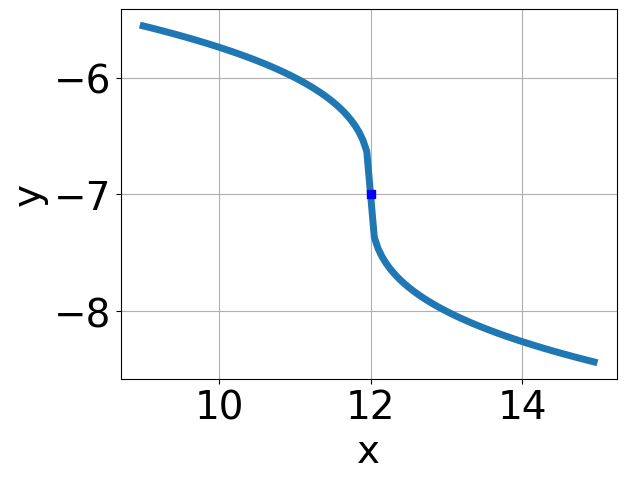
\includegraphics[width = 0.3\textwidth]{../Figures/radicalEquationToGraphCB.png}\item 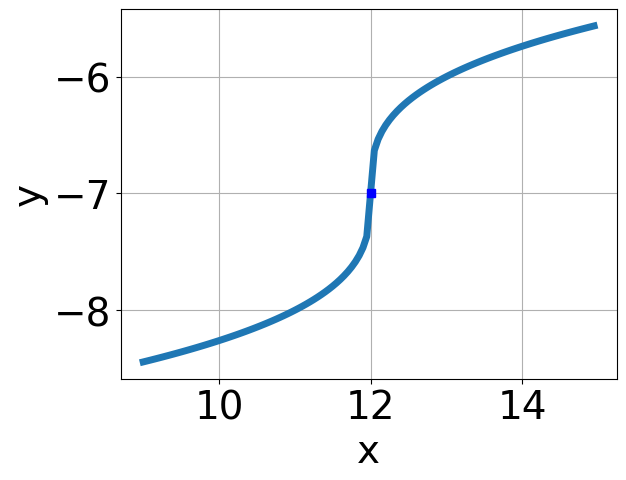
\includegraphics[width = 0.3\textwidth]{../Figures/radicalEquationToGraphDB.png}\end{multicols}\item None of the above.
\end{enumerate} }
\litem{
Solve the radical equation below. Then, choose the interval(s) that the solution(s) belongs to.\[ \sqrt{-3 x - 9} - \sqrt{-9 x - 3} = 0 \]\begin{enumerate}[label=\Alph*.]
\item \( x \in [0.76,1.1] \)
\item \( x_1 \in [-4.14, -2.2] \text{ and } x_2 \in [-2,0.6] \)
\item \( x \in [1.6,3.24] \)
\item \( x_1 \in [-4.14, -2.2] \text{ and } x_2 \in [-0.2,1.6] \)
\item \( \text{All solutions lead to invalid or complex values in the equation.} \)

\end{enumerate} }
\litem{
Solve the radical equation below. Then, choose the interval(s) that the solution(s) belongs to.\[ \sqrt{24 x^2 - 36} - \sqrt{5 x} = 0 \]\begin{enumerate}[label=\Alph*.]
\item \( x_1 \in [1, 1.27] \text{ and } x_2 \in [1.33,5.33] \)
\item \( \text{All solutions lead to invalid or complex values in the equation.} \)
\item \( x_1 \in [-1.26, -1.08] \text{ and } x_2 \in [1.33,5.33] \)
\item \( x \in [1.3,1.36] \)
\item \( x \in [-1.26,-1.08] \)

\end{enumerate} }
\litem{
Solve the radical equation below. Then, choose the interval(s) that the solution(s) belongs to.\[ \sqrt{72 x^2 + 12} - \sqrt{60 x} = 0 \]\begin{enumerate}[label=\Alph*.]
\item \( x_1 \in [-0.55, -0.29] \text{ and } x_2 \in [-0.42,0.44] \)
\item \( x \in [0.32,0.37] \)
\item \( x_1 \in [0.32, 0.37] \text{ and } x_2 \in [0.35,1.35] \)
\item \( x \in [0.49,0.62] \)
\item \( \text{All solutions lead to invalid or complex values in the equation.} \)

\end{enumerate} }
\end{enumerate}

\end{document}